\documentclass[12pt]{article}
\usepackage{hyperref}
\hypersetup{colorlinks=true,urlcolor=blue}
\usepackage{listings}
\usepackage{geometry}
\geometry{margin=1in}
\usepackage{graphicx}
\graphicspath{ {./} }
\lstset{language=Python,keywordstyle={\bfseries \color{purple}}}
\begin{document}
\title{BMI 203: Algorithms - Final Project}
\author{Laurel Estes}
\maketitle
\section*{Part I: Neural Network Learning an 8-3-8 Encoder}
I constructed a NeuralNetwork Class that consists of an array of Layer Class objects and contains feedforward and backpropagation methods. The Layer Class defaults to a sigmoidal activation function, but other activation functions can be passed in; the NeuralNetwork Class, however, as currently implemented, explicitly uses the derivative of the sigmoid function in its backpropagation function, and will not work with other activation functions. Layers are represented as 2D matrices of weights, with rows corresponding to nodes in the layer and columns corresponding to inputs to that layer. Based on various resources suggested to the class, Xavier initialization is used for the random weights (see code comments for specific links).
\par This NeuralNetwork code is able to learn a viable 8-3-8 encoder, as represented in \verb|nn/encoder.py|, which contains a function that generates a trained 8-3-8 encoder. The default parameters in \verb|make_838_encoder| represent the best values of the neural network hyperparameters found via a grid search conducted in \verb|nn/__main__.py|. Pytest was used to validate this implementation: the tests in \verb|test/test_nn.py| are designed to ensure that the NeuralNetwork Class is working correctly independent of a specific learning task, whereas the tests in \verb|test/test_encoder.py| validate that the implementation I created is capable of learning an 8-3-8 encoder to within an error of 0.1 per digit after 10,000 training iterations. A screenshot of the terminal output representing this is below:
\begin{figure}[h!]
\centering
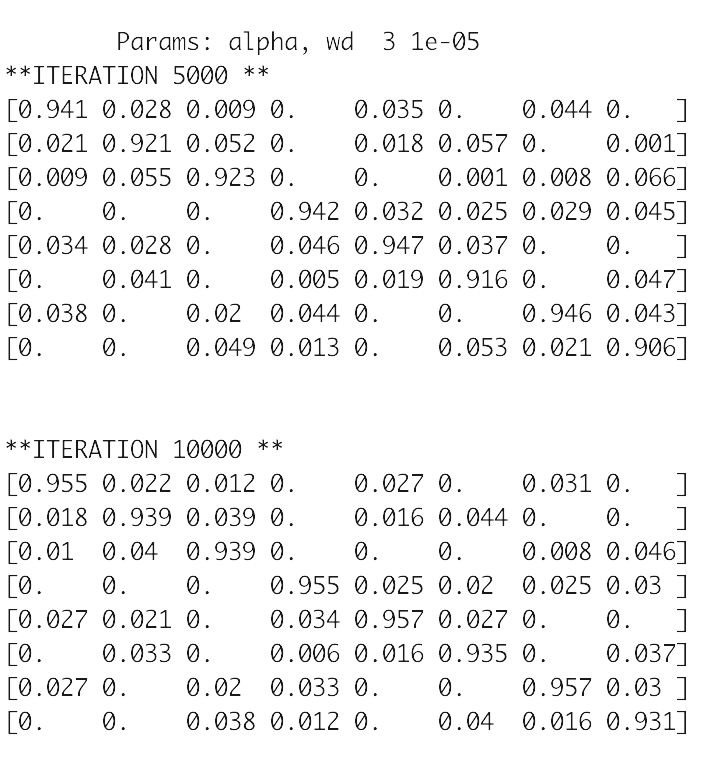
\includegraphics[width=0.3\textwidth]{838_encoder.png}
\end{figure}
\section*{Part II: Learning Procedure for Rap1 Recognition Sites}
\subsection*{Preprocessing}
First, the upstream yeast genomic data fasta file was processed into a list of 17-bp chunks that were reverse-complemented (doubling the total size of the set), then screened for matches with any of the known positive sequences in rap1-lieb-positives.txt, then written out to rap1-lieb-constructed-negatives.txt. Then, the minimum hamming distance between each negative sequence and any of the positive sequences was calculated (and plotted in a histogram, sorry it's kind of ugly because I got the bin sizes wrong):
\begin{figure}[h!]
\centering
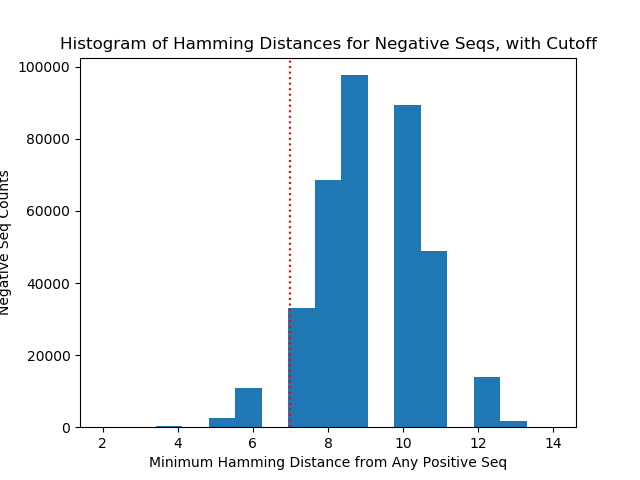
\includegraphics[width=0.4\textwidth]{HammingDistHistogram.png}
\end{figure}
The hamming distance cutoff of 7 bp away was chosen qualitatively based on the shape of the histogram, and all the negative sequences were split into either rap1-lieb-close-negatives.txt (if the hamming distance was less than or equal to 7) or rap1-lieb-far-negatives.txt (if the hamming distance was greater than 7). The theory behind this processing was that there is far too much negative data ($>300$k) relative to the positive data (137) to be able to reasonably use all of it to train the model, and that the most interesting/useful/information-rich sequences for our purpose will be those that are {\it close} to the positives but not actually hits. This hamming distance cutoff leaves around 46k `close negatives'. 
\subsection*{Featurization}
To featurize the sequences into a numeric form that the classifiers can interpret, I used flattened one-hot matricies, an approach I read about in this article: \url{https://www.scirp.org/journal/PaperInformation.aspx?PaperID=65923}. By splitting the sequence into a sparse 2D array of k-mers where the single '1' per column corresponds to the k-mer present at that location (essentially the same structure as the inputs to the 8-3-8 encoder above!), we ensure that the k-mers are considered to be orthogonal dimensions. Conversing with some of my peers has suggested that for this application, naive ordinal featurization (aka A = 0.25, T = 0.5, C = 0.75, and G = 1.0 etc.) is actually almost as effective, which is interesting to note. Given more time, I would have liked to test featurization using 2-bp k-mers, but in this case, I just used single base pairs at every position, so each input 17-bp sequence becomes a 4x17 2D array, which is then flattened. 
\subsection*{Model Selection and Cross-Fold Validation}
Given the extreme imbalance (3 orders of magnitude) in the positive and negative classes in our data, some method of undersampling and/or oversampling seemed required to create training datasets that would not simply cause the classifier to always guess the majority class. I decided to employ multiple different sampling methods, then use stratified k-fold cross-validation to determine the best parameters from a small grid search of model choice and structure for the dataset created by that sampling method. 
\par As detailed in the code comments in \verb|tf/__main__.py|, the datasets I created are as follows:
\begin{itemize}
	\item Undersampling, using all 137 positives, a 1:2 ratio of pos:neg sequences, and a 90\%-10\% split of close negatives and far negatives 
	\item Oversampling, using 10,000 total samples, a 1:5 ratio of pos:neg sequences (with the positives bootstrap-upsampled), and 100\% close negatives
	\item Combination Over/Under-Sampling, using 500 positives, a 1:2 ratio of pos:neg sequences, and a 90\%-10\% split of close negatives and far negatives 
	\item Combination Over/Under-Sampling as above but with a 1:5 ratio of pos:neg sequences
	\item Combination Over/Under-Sampling as above but with a 1:10 ratio of pos:neg sequences and a 99\%-1\% split of close negatives and far negatives  
\end{itemize}
Each of these datasets was split into 3 stratified folds of train/test data. Stratified folds were created because the ratios were still not 1:1 and the dataset sizes were relatively small for a machine learning problem (100s to 10,000 sequences), so maintaining the original ratio of positives to negatives to avoid the effects of unusual fold composition seemed relevant and important. Once the data had been split, for each fold, I trained four different classifiers across a range of parameters to determine the best classifier and classifier parameter for that specific dataset. To save time and effort, since I had already made a working neural network implementation from scratch in Part I, I used the \verb|scikit-learn| package for the classifiers and attendant functions for this task. The four classifiers tested were: an MLP using the 'adam' stochastic gradient descent variant algorithm, an MLP using the LBFGS algorithm (a quasi-Newtonian method which the sklearn documentation indicated is sometimes better for smaller datasets), a K-Nearest Neighbors classifier using uniform weighting, and a K-Nearest Neighbors classifier using weighting proportional to distance. I limited my search of hyperparameters to just the hidden layer structure (for the MLPs) and the number of nearest neighbors (for the KNNs). Based on the paper I presented in class, I used 2-layer pyramidal structures for my hidden layer options, e.g. (100,10). The ROC-AUC score for each classifier and parameter combination was calculated for each fold, and the classifier/parameter combination that had the highest mean ROC-AUC score across all 3 folds was returned as the best classifier for that dataset. 
\par In general, the highest-performing classifier for each dataset performed {\it very} well, with ROC-AUC scores $>0.9999$. This seemingly good result does make me wary of overfitting, which prompted me to ensemble the best classifiers in order to make the final predictions.

\section*{Part III: Predicting Rap1 Recognition Sites}
Once the best classifier for each dataset had been obtained, predictions on the \verb|rap1-lieb-test.txt| sequences were made by an ensemble of these best classifiers. Each classifier in its own training regime had the opportunity to overfit to the unavoidably small number of (unique) true positives in its training data; however, since the exact dataset that each classifier was trained on was different, the overfitting should occur in different `directions' for each one. Therefore, ensembling the classifiers together should decrease the overfitting overall, since the different `directions' will (at least partially) cancel out when averaged together.
\par When each optimal classifier is trained on the entirety of its particular dataset, and then used to predict the pos/neg class of the test sequences in rap1-lieb-test.txt, two populations of classifiers stood out to me. The two classifiers trained on the smallest datasets (undersampling and combined-1:2) seem to have less certain predictions (closer to 0.5 than 0 or 1) and more positive predictions, and they tend to agree on their predictions. 
\par Despite the general simplicity of the dataset, I am suspicious of my undersampling classifier, since all of the MLP classifiers performed essentially equally in that test and the 'best' returned classifier is the one only with a single hidden layer of 10 nodes. The flip side to that suspicion, however, is that those two classifiers are the ones trained on the most balanced of the datasets (1:2 ratio instead of 1:5 or 1:10), which could be causing an artifical inflation of negative results in the other classifiers. I chose to leave the undersampling classifier out of my final ensemble, but did the pre-averaged ensemble classifications for all five classifiers in individual_predictions.txt. Had I more time, I would have done a holdout within the given training data to try to determine which population of classifiers was more on track overall. 
\par The final ensemble classification probabilities are given in ensemble_predictions.txt
\section{Github Repository}
All of the code used in this assignment is on Github: \url{https://github.com/laueste/algorithms-ucsf-2019}
\end{document}